\chapter{Overall Description}

\section{Product perspective}
\subsection{Class diagram}
In figure \ref{fig:class_diagram} is presented the high-level overview of the CKB system. \newline
The main elements are:
\begin{itemize}
    \item User: that can be either student or educator. It is identified by a unique username.
    \item Student: represent the personal profile of a student. It contains the earned badges, the number of battle won, and all tournament rankings.
    \item Team: identifies a group of students that can join a battle. Students must form a team in order to participate in a battle, even if it is formed by one.
    \item Tournament: identifies a tournament. It contain all useful information as well as all needed method(s) that allow the educators to create it and the students to enroll into it. It also contains the final ranking of all participants.
    \item Battle: identifies a battle. It contain all useful information as well as all needed method that allow the educators to create it and the team of students to join it. It also contains the ranking of all teams.
    \item Evaluator: it contains all files and methods that are necessary for both the automatic and manual evaluation.
    \item Badge: represent a badge with a title, description and a set of rules that regulates how a student can earn the badge. All rules must be checked in order to give the badge to the student.
    \item Rule: represent a rule. It contains the method(s) that check whether a student can receive the badge.
\end{itemize}

\begin{figure}[H]
    \centering
    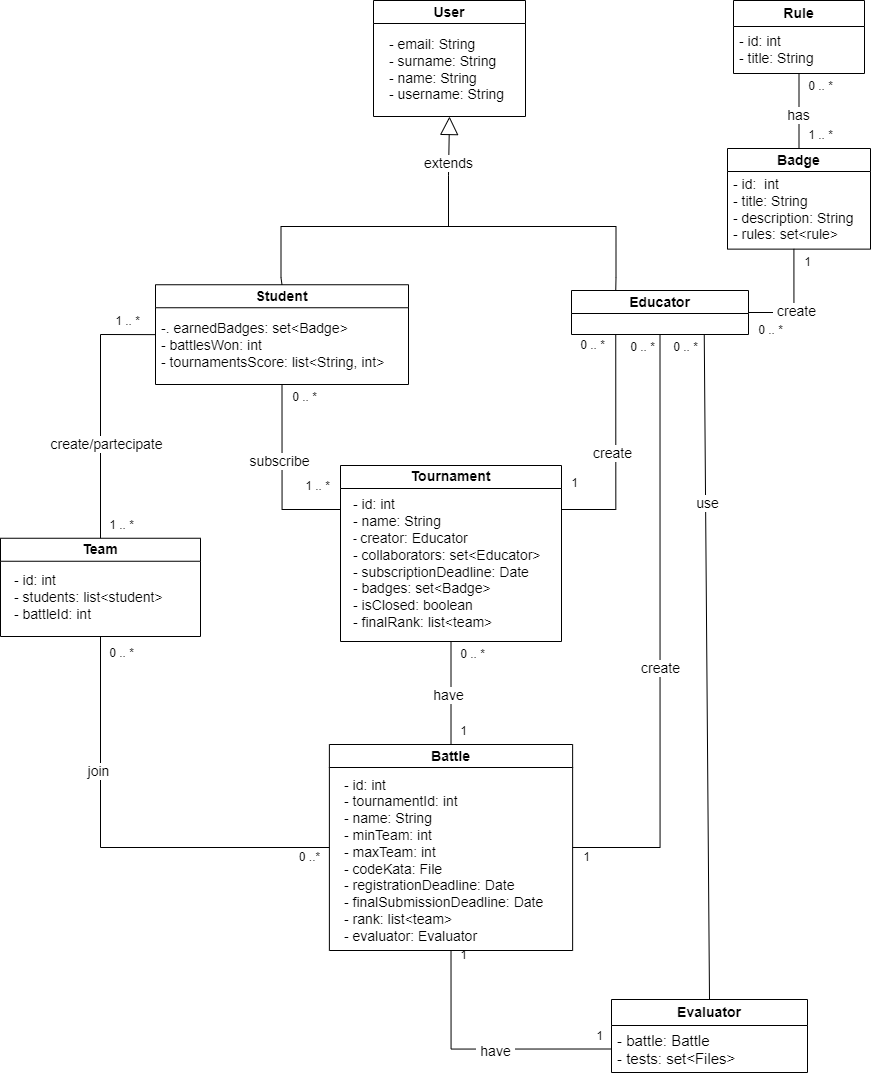
\includegraphics[scale=0.5]{images/class_diagram.png}
    \caption{Domain class diagram}
    \label{fig:class_diagram}
\end{figure}
\clearpage

\subsection{State diagrams}
The following state diagrams describe the behaviour of the system focusing on the evolution over time of some particular aspects. 

\subsubsection*{Tournament state diagram}
The state diagram in figure \ref{fig:tournament_state} represent the evolution of a tournament, from its creation to its closure. \newline
As soon as an educator creates a new tournament with all necessary information, the enrollment stage opens and students can spontaneously register until the deadline expires. \newline
While the tournament is ongoing educators, who have the permits, can create new battles (further explanation below). It is possible that a tournament has no active battles, but it is still ongoing, for this reason we distinguished the two states clearly. \newline
Only when all the battles are finished the creator can close the tournament, and the final ranking will then be available.
\begin{figure}[H]
    \centering
    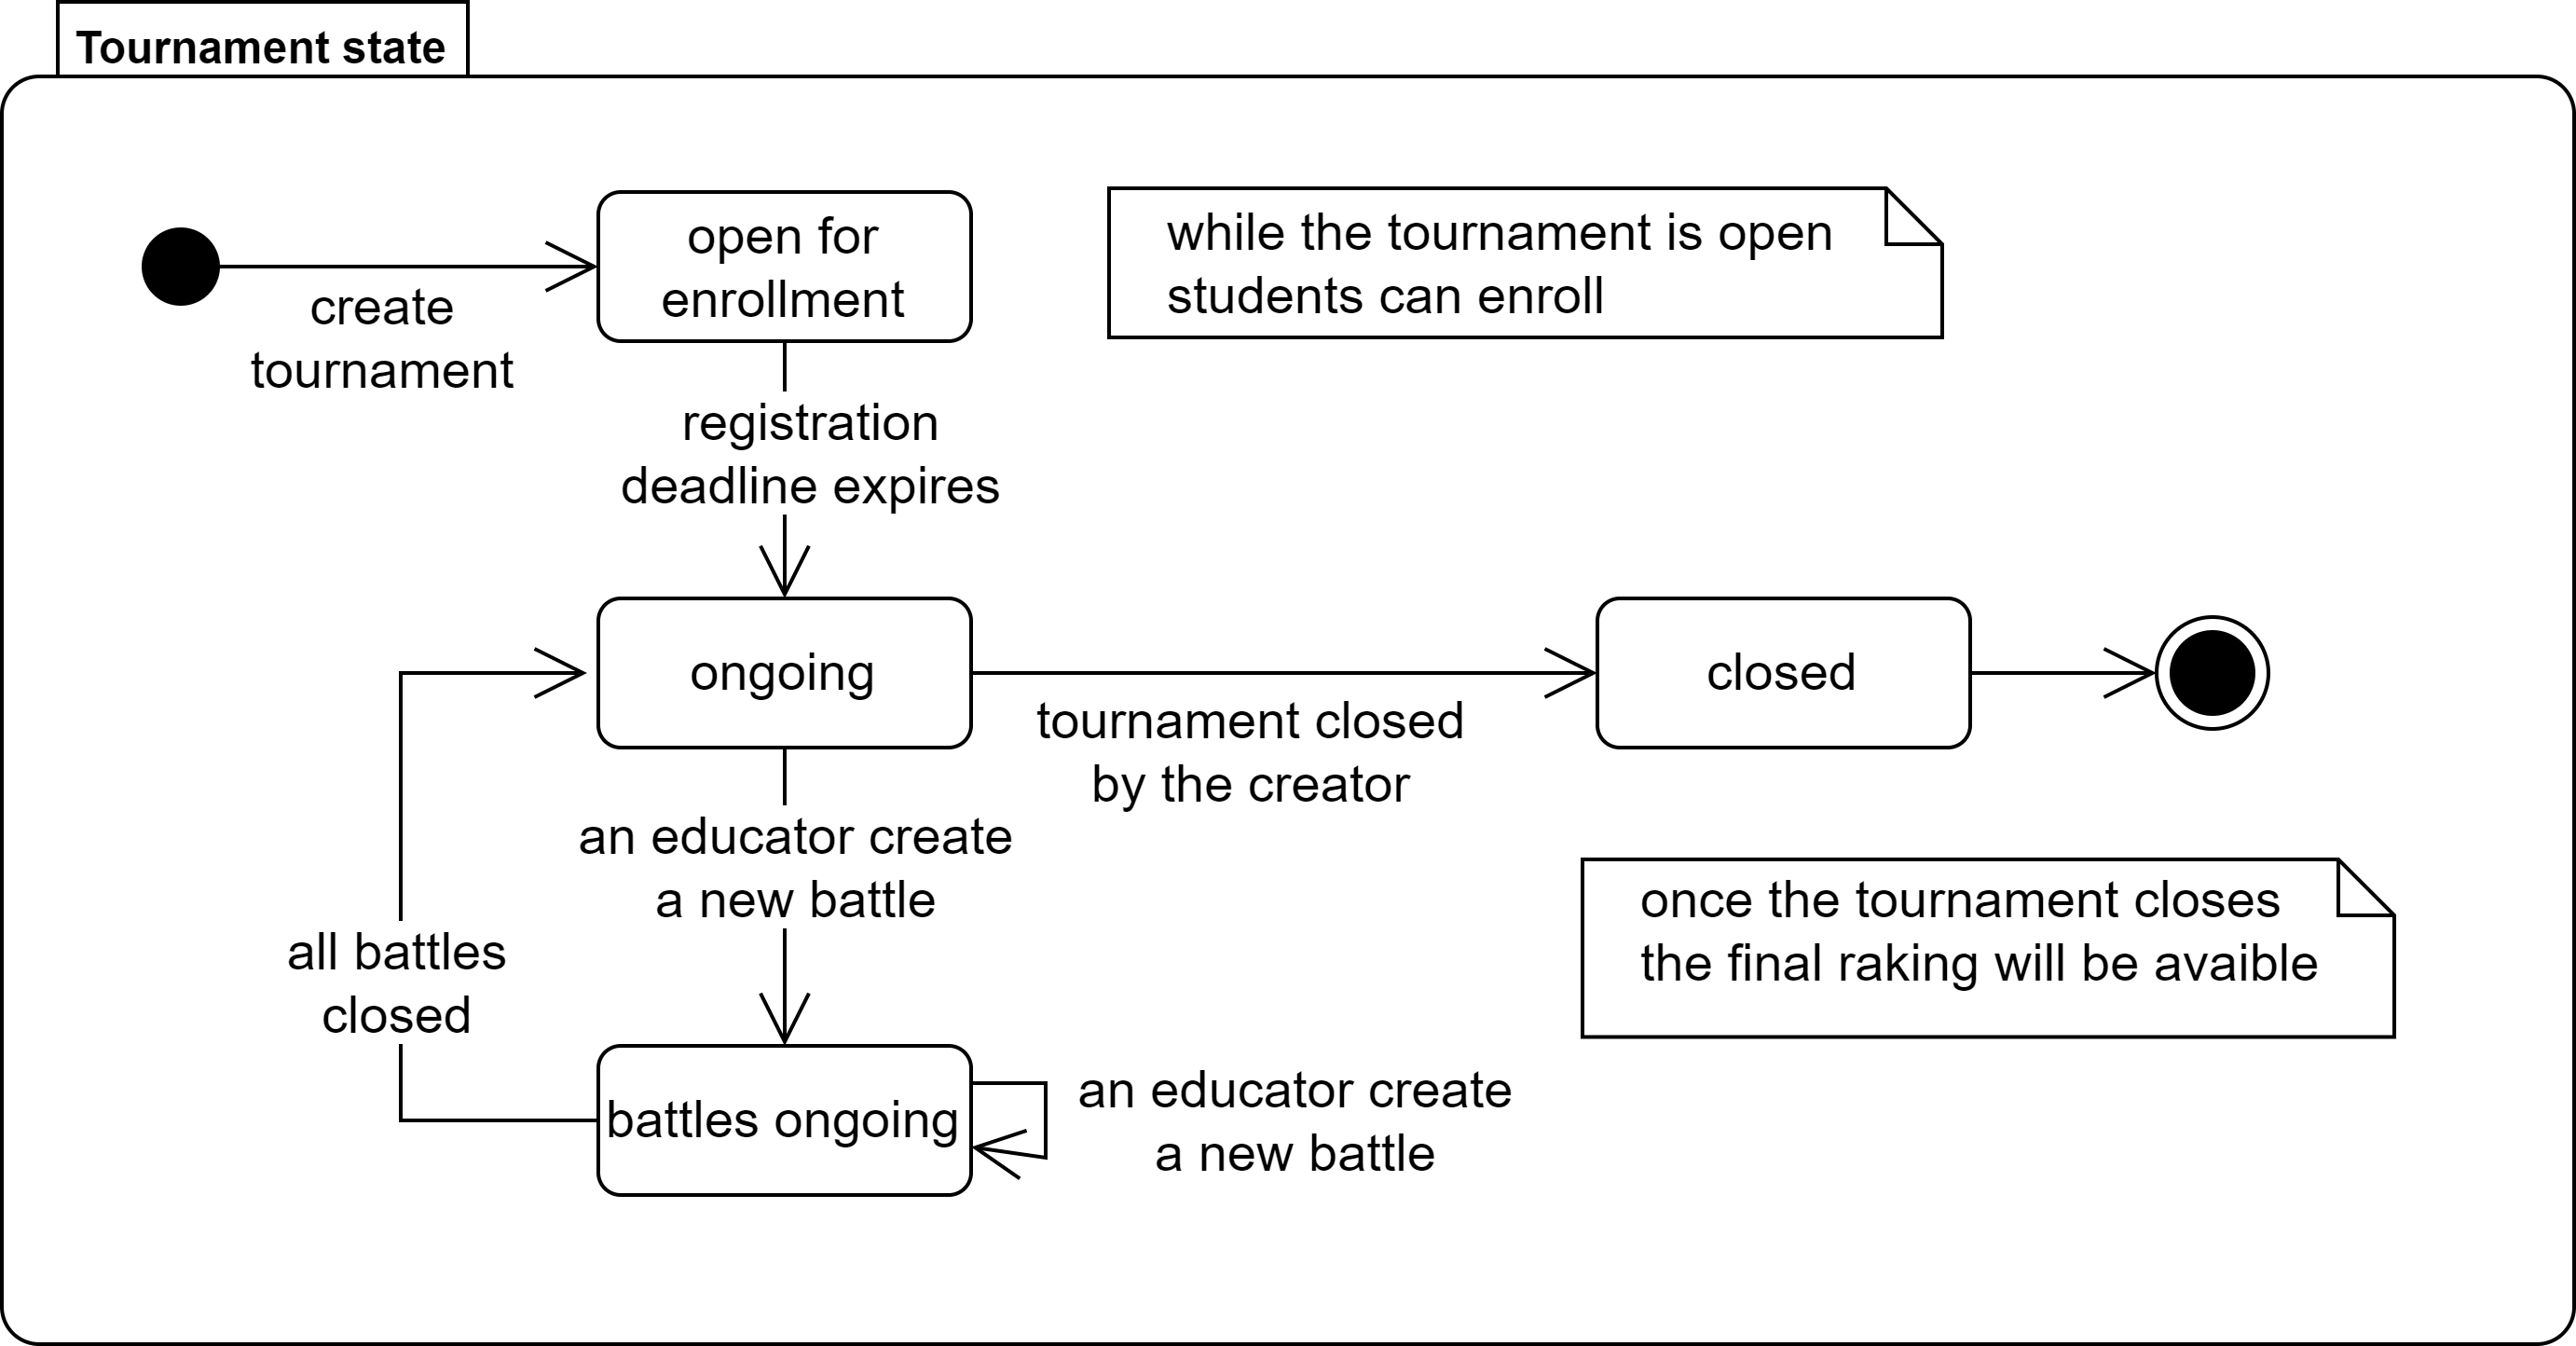
\includegraphics[scale=0.5]{images/tournament_state.png}
    \caption{Tournament state diagram}
    \label{fig:tournament_state}
\end{figure}

\subsubsection*{Battle state diagrams}
The state diagram in figure \ref{fig:battle_state} represent the evolution of a battle, from its creation to its end. \newline
As soon as an educator create a new battle with all necessary information, the enrollment stage opens. Students, who are registered to the tournament in which this battle belongs, can enroll with a team (further explanation below). \newline
When the registration deadline expires, the enrollment stage closes, the GitHub repository is automatically created and the battle is ongoing. As soon as a new push is available in a repository of a team the automatic evaluation is performed, and the ranking is updated. \newline
When the final submission deadline expires the battle ends and a consolidation stage opens, during which the educator can perform the manual evaluation (if needed). When the educator finishes he/she can close the consolidation stage and the ranking will be available.
\begin{figure}[H]
    \centering
    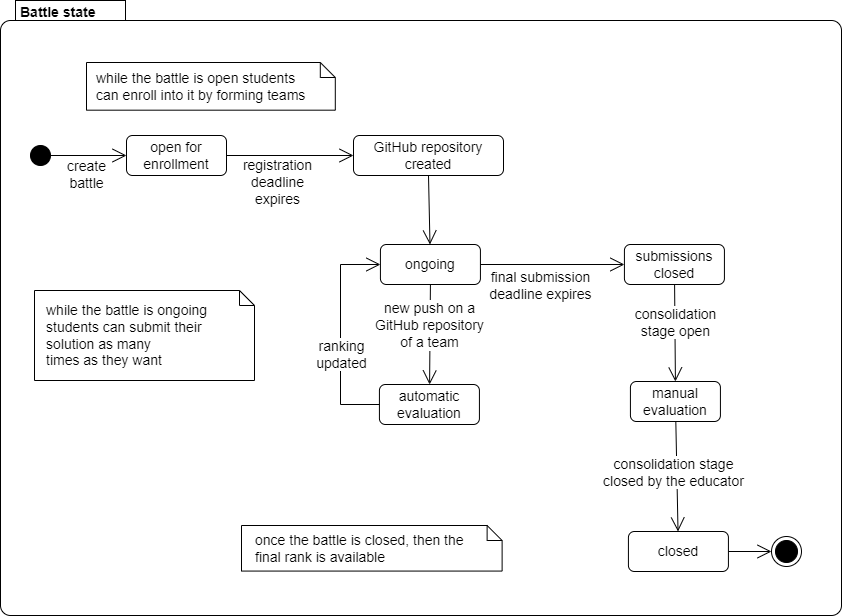
\includegraphics[scale=0.5]{images/battle_state.png}
    \caption{Battle state diagram}
    \label{fig:battle_state}
\end{figure}

\subsubsection*{Team state diagrams}
The state diagram in figure \ref{fig:team_state} represent the evolution of a team, from its creation to its end. \newline
When a student who is enrolled in a tournament wants to participate in a battle he/she must create a team. The creator can send infinite invitations, and the firsts to accept will be added to the team. As soon as the team reach the maximum value of students, it is complete and all other invitations sent before will not be useful. \newline
As soon as the battle registration deadline expires the team formation closes. If the team has reached the minimum required value it is complete and can participate to the battle. Otherwise it will be eliminated. \newline 
If all invitations are declined the creator have the possibility to eliminate the team. 
If the creator create the team by error, he can eliminate it. This is necessary because a creator is not allowed to join another team by accepting an invite.

\begin{figure}[H]
    \centering
    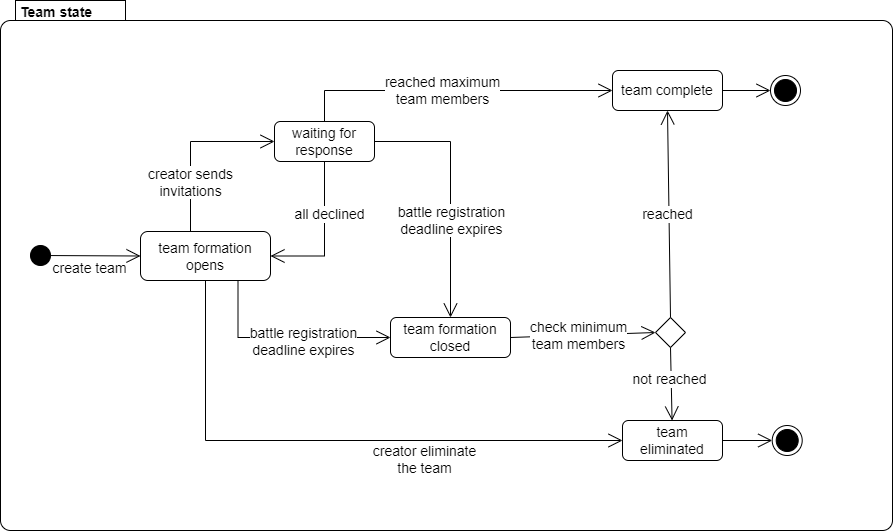
\includegraphics[scale=0.5]{images/team_state.png}
    \caption{Team state diagram}
    \label{fig:team_state}
\end{figure}
\clearpage

\subsection{Scenarios}\label{desc:scenarios}
In this section we will analyze all possible scenarios that can occur in using the CKB platform.

\subsubsection{Scenario 1: Users registration}
Mario is a professor and wants to challenge his students, so he choose the CKB platform. He creates a personal account by inserting some personal information and then get a confirmation e-mail about the creation of a new account. He now can be able to create tournaments and battle. \newline
Peach is a computer science student and wants to improve her software development skills. She learns about the CKB platform from her professor, and decide to create an account to be able to participate to battles. The platform request some personal information and then she get a confirmation e-mail about the creation of his new account. She now have a personal profile where every other user can see her progress, in terms of badges earned, battles won, and tournament rankings. \newline
In both cases the platform request some personal information such as name, surname, username, password, e-mail and the role, that can be student or educator. The account is created after the user clicks on the link sent in the confirmation e-mail. All future notifications will be sent through that e-mail. \newline
Every registered user can log-in with username and password any time, in order to access the personal dashboard and use the CKB platform.

\subsubsection{Scenario 2: Tournament and battle creation}
Mario, that is a registered educator, wants to create a new tournament called "Super Smash". He open the CKB platform, log-in, and from his personal dashboard he select the option "create new tournament". He then follows all the steps that allows him to set a registration deadline and a minimum and maximum number of participants. He can then invite other educators to create battles within his tournament. \newline
Mario invites Luigi to his tournament by adding his username to the list of collaborator. Luigi will be notified by e-mail, and if interested have to join the tournament. \newline
Luigi, that is also a registered educator, wants to create a new battle in Mario's tournament. He open the CKB platform, log-in, and from his personal dashboard he select "Super Smash" from the list of his tournaments.
He then select the option "create new battle" and follows all the steps that allows him to upload the code kata, set a registration deadline, minimum and maximum number of students per group and a final submission deadline.
The tournament "Super Smash" with the first battle are now open, in the list of all ongoing tournaments. \newline
When all ongoing battles within the tournament have finished Mario can close it. Then the CKB platform will publish the final tournament ranking when is available and send a notification to all enrolled students.

\subsubsection{Scenario 3: Students team formation}
Peach, that is a registered student, wants to join a tournament. She open the CKB platform, log-in, and from her personal dashboard she is able to see the list of all ongoing tournaments. She selects a tournament and, if the subscription phase is still open, she enrolls.
Daisy enrolls in the same tournament as Peach. \newline
Peach decides to form a team. She can invite students up to the maximum number allowed. She has a limited number of invitations, and if someone does not accept the invitation within a fixed time, she can re-send the invite to someone else.
She sends the invite to Daisy and Toad by adding their username in the team. They will receive a notification by e-mail, and if interested can join the team. Toad decided to join, while Daisy decline the invite. \newline
If the team reach the minimum number of participants for the battle by the registration deadline, they can compete. \newline
\textbf{A team does not reach the minimum number of participants:} Let's say that the minimum number of participant for the  previously mentioned battle is 3, in this case Peach can re-send the invite to another student but she forgot and the registration deadline expires.
Peach's team cannot compete in the battle, therefore their score will be automatically 0.

\subsubsection{Scenario 4: Real-time battle progress}
Peach has formed a valid team for a battle within a tournament. The CKB platform has automatically created a GitHub repository with all the essential elements for the resolution of the battle, and send a link to all enrolled students.
Peach and her team have to fork this repository and set up an automated workflow 
through GitHub Actions. At each pushed commit the platform automatically update the total score of the team. The team is also able to see the current ranking evolving during the battle, so they can improve their solution to get a better rank.\newline
\textbf{Students push the solution in a different language:} Every submission that does not use the language specified in the project description will not be evaluated, therefore the team will get a score of 0.  \newline
\textbf{Students push the solution after the deadline:} Every submission after the deadline is ignored, therefore the team will get a score of 0. 

\subsubsection{Scenario 5: Manual evaluation}
After the final submission deadline of a battle expires, a consolidation phase open. During this phase Luigi, that is the creator of the battle, can optionally assign a personal score to each student that will be added to the total score of the entire team.
As soon as Luigi has finished to evaluate all students, he will end the consolidation phase, and when the ranking are available all students will be notified.\newline
\textbf{The score exceed the maximum value:} Luigi can make a mistake and assign a score to a student making the overall team score higher than 100. In this case the score will be automatically cut off to 100.

\subsubsection{Scenario 6: Gamification badges management}
Mario, that is a registered educator, wants to create a new badge that is earned by the student who wrote the most lines of code. From his personal dashboard he select the option "create new badge", then he has to specify the name, a description and one or more rules that regulates if a student is eligible to get that badge. In this case the name will be "Top Writer" and it will be awarded to the student who wrote the most lines of code within a battle. \newline
Peach, that is a student, aspires to earn the "Top Writer" badge, and so she heavily contributed on the last battle. At the end of the battle the CKB platform automatically checks if any student is eligible for a badge, and Peach is assigned the "Top Writer", which will appear on her CKB profile.

\subsubsection{Scenario 7: Visualize student profile}
Mario is logged and want to check the profile of Luigi, in order to do this, he write the username of Luigi in the search-bar, will be visualized the resuming information about Luigi, including all the badges that he had collected.

\clearpage

\section{Product functions}\label{desc:prodFunc}
In this section are explained the main functions that the CKB should provide to its users.
\subsection{Sign Up and Login}
These function will be available for all user.\newline All users can create a new profile by the sign up function. Each profile is uniquely identified by a username. Each user will be ask to provide an email, a password and role (student or educator). \newline
A login can occur every time by the use of username (or email) and password.

\subsection{Create and manage a tournament}
This function will be available only for educators. \newline
Each educator can create a new tournament and invite other colleagues to create battles within that tournament. At the creation the educator must specify the subscription deadline. 
A tournament can then be closed by its creator, and as soon as the final tournament ranking is available the CKB platform notify all students subscribed.

\subsection{Create a battle within a tournament}
This function will be available only for educators. \newline 
An educator can create a new battle in a tournament only if he/she created it or he/she have been invited to collaborate by another colleague.
The system allow the educator to specify: 
\begin{itemize}
    \item code kata, that consist in the description and software project including test cases and build automated scripts.
    \item minimum and maximum number of students per group.
    \item registration deadline.
    \item final submission deadline.
\end{itemize}
The educator has to specify the languages in which the submission can be made.
When the registration deadline expires, the CKB platform creates a GitHub repository that contain the code kata, and sends the link to all the students enrolled in the battle.

\subsection{Subscribe to a tournament}
This function will be available only for students. \newline When a new tournament is created all registered students are notified and can subscribe within a given deadline.

\subsection{Join a battle}
This function will be available only for students. \newline When there is an upcoming battle in a tournament all subscribed students are notified. Each student can join a battle only with a team, even made up of only one student if it is allowed. 

\subsection{Create a team}
This function will be available only for students. \newline
Teams are formed by invite. The creator is able to send infinite invitations, and the firsts to accept will be added to the team.  \newline
The invite will be received by e-mail, and the recipient must click on the right link if he/she wants to accept or decline. The student has 24h to respond to an invite, otherwise it will be automatically declined. \newline
The creator is not allowed to accept other invitations. If all invitations are declined the creator can eliminate the team.

\subsection{Automatic scores updates}
When the students push a new commit into the main branch of the GitHub repository, the CKB platform automatically analyze it and runs the tests to calculate and update the battle score of the team.\newline
The score of each battle is automatically evaluated in the following ways:
\begin{itemize}
        \item functional aspects, measured in terms of number of test cases passed over all test available. The higher the better.
        \item time passed between the registration deadline and the last commit. The lower the better.
        \item quality level of the source, extracted through static analysis tools based on aspects chosen by the educator when creating the battle. 
\end{itemize}

\subsection{Manually scores updates}
When a battle ends, a consolidation stage open. The creator of the battle is able to optionally perform a manual evaluation for each student enrolled.
Once the educator has evaluated all students he can end the consolidation, and when the final battle ranking is available all enrolled students will be notified.

\subsection{View all rankings}
Every user can see the list of ongoing tournaments and the corresponding ranking (that compares all subscribed students' performance) in the CKB platform.
At the end of each battle the personal tournament score of each student is automatically updated ad the sum of all battle scores received. 

\subsection{View a student profile}
Every user can view a profile of a student by searching for his/her username. In each profile are shown badges earned, battles won, and tournament rankings. 

\subsection{Create and manage gamification badges}
This function will be available only for educators. 
\newline A badge can be created by specifying a title and at least one rule that must be satisfied to achieve it. Each badge is then automatically assigned to one or more students by checking the validity of the rules. Educators can also create new variables that represent relevant information for scoring. A variable is identified by a unique name and a measurement unit, that can be selected by a list of predefined (e.g. integer, float, date, ..).

\clearpage

\section{User characteristics}
Each user must have a profile to be able to use the CKB platform.
There are two different type of users:
\begin{itemize}
	\item \textbf{Students}:
	    The students are the primary users of the CKB platform. They range from beginners to advanced learners. Each student has a personal profile that display their badges earned, battles won, and tournament rankings. 
	\item \textbf{Educators}: 
		The educators can creates and manages tournaments and/or battles. They challenge the students and then evaluate and grade them based on their submissions. An educator must be officially recognized as he/she should have the adequate knowledge.
\end{itemize}

\section{Assumptions, dependencies and constraints}

\subsection{Domain assumptions}
In this section are listed all assumption made for the domain in which the system operates. These are conditions that the system take for granted because they are external to it but influence its behaviour.
\begin{enumerate}[label=\textbf{DA.\arabic*}]
        \item \lbl{da: internet} {Users must have internet connection to interacts with the CKB platform.}
        \item \lbl{da: eduQual} {Educators must be qualified and experienced in software development and related fields.}
        \item \lbl{da: correctCode} {The uploaded "code kata" by the educators must be correct and complete.}
        \item \lbl{da: GitHubAccount} {Students must have a GitHub account to be able to deliver a solution.}
        \item \lbl{da: GitHubFork} {Students must fork the GitHub repository created by the CKB platform and set up an automated workflow through GitHub Actions.}
        \item \lbl{da: devEnv} {Students must have a development environment with the necessary software tools and libraries to complete code kata battles.}
        \item \lbl{da: autWorkFlow} {The automatic workflow correctly trigger the CKB platform in order to evaluate the new commit.}
        
        
\end{enumerate}

\subsection{Constraints}
In this section are presented general considerations about limitations on the systems.

\subsubsection*{Regulatory policies}
All users information will be processed in according with the GDPR, and e-mail addresses won't be used for commercial purposes.
